% ---------------------------------------------
% Autor:        Melanie Windrich, Timo Wilgen 
% Vorlage:      Daniel Fötsch, Sven Feja, Eckhard Anders
% Beschreibung: Hauptdatei der Diplomarbeit
% Dateiname:    main.tex 
% Projekt:      Diplomarbeit
% erstellt am:  31.10.2010
% geändert am:  06.12.2018
% SVN:		$Id$
% ---------------------------------------------
\documentclass[
	pdftex,			% Seitenangaben ins pdf schreiben
	11pt,			% Schriftgröße 12pt
	a4paper, 		% Layout für DIN A4
	twoside, 		% Layout für zweiseitigen Druck
	%fleqn,			% Formeln links eingerückt (default mittig)
	BCOR=2cm,		% Binderandkorrektur
	DIV=11,			% a little more room on page
	listof=totoc
]{scrbook} 

% Packages
\usepackage{scrhack}           % KomaScript compatibility hacks (e.g. for listing)
\usepackage[utf8]{inputenc}    % Paket für Eingabekodierung 
\usepackage[ngerman]{babel}    % Unterstützung für Deutsch (neue Rechtschreibung)
\usepackage[T1]{fontenc}       % T1-kodierte Schriften, korrekte Trennmuster fuer Worte mit Umlauten
%\usepackage{lmodern}		   % benutze Latin Modern als Standardschriftart
\usepackage{mathptmx}		   % benutze Times als Standardschriftart
\usepackage{helvet}		       % Serifenlose Schriftart
\usepackage{ifpdf}		       % Parameter zur Erkennung des Kompilierungstyps
\usepackage{listings}		   % Code einbinden
\usepackage{microtype} 		   % unterbindet full boxes durch bessere Anpassung der Schrift 
\usepackage{bibgerm}		   % Deutscher Biobliographiestil (geralpha)
\usepackage{amssymb}		   % mathematische Symbole \mathbb{N} z.B.
\usepackage{nomencl}		   % Abkürzungsverzeichnis
\usepackage{xspace}		       % Leerzeichenproblem bei Commands lösen
\usepackage{setspace}		   % benötigt für Zeilenabstände
\usepackage{booktabs}		   % \toprule für Tabellen
\usepackage{enumitem}
\usepackage[hyphens]{url}
\usepackage[pdftex]{graphicx}  % Einbinden von Grafiken
\usepackage[pdftex]{color}     % Einbinden von Farben
\usepackage[pdftex]{xcolor}
\usepackage[pdftex]{hyperref}  % Einbinden von Verlinkung
\usepackage{todonotes}		   % \todo{} befehl [disable] zum deaktivieren
\usepackage{pdfpages} 	       % Einbinden von pdf
\usepackage{cite}		       % Für bibtex Parsing unter Windows
\usepackage{blindtext}
\usepackage{amsmath}		   % AMS Mathe und Symbolpakete für mehr Möglichkeiten
\usepackage{amsfonts}
\usepackage{amssymb}
\usepackage{verbatim}          % \begin{comment}, \end{comment}


\usepackage{multirow}		   % Zeilen in Tabellen zusammenfassen (http://tug.ctan.org/tex-archive/macros/latex/required/graphics/grfguide.pdf)
\usepackage{hhline}		       % Horizontale Linien in Tabellen feiner gestalten
\usepackage{longtable}

% Unterabbildungen können mit dem subfig-Paket realisiert werden.
% (z.B. Abb. 1a) (http://tug.ctan.org/tex-archive/macros/latex/contrib/subfig/subfig.pdf)
\usepackage{subfig}

% Großartige Möglichkeiten um Grafiken direkt in LaTeX zu erzeugen bietet Tikz 
% (http://mirror.ctan.org/graphics/pgf/base/doc/generic/pgf/pgfmanual.pdf und http://www.statistiker-wg.de/pgf/tutorials.htm)
\usepackage{tikz}		% 
\usetikzlibrary[shapes.misc,shapes.geometric,arrows,decorations.pathmorphing,backgrounds,fit,positioning]

% \setlength{\headheight}{10mm}
% \setlength{\headsep}{8mm}  

% \setcounter{secnumdepth}{3}           % Globale Tiefe im Dokument
% \setcounter{tocdepth}{3}              % Tiefe der Numerierung im Inhaltsverzeichnis
\renewcommand{\topfraction}{0.99}
\renewcommand{\textfraction}{0.01}
% Die vorangegangenen Befehle sind noetig, damit grosse Objekte nicht
% erst auf der letzten Seite erscheinen... (siehe Kopka-Buch S. 170)

\setcounter{topnumber}{9}
\setcounter{totalnumber}{9}
% Damit mehr Tabellen/Abbildungen auf eine Seite passen. (S. 170)

% Hurenkinder und Schusterjungen verbieten
\clubpenalty = 10000
\widowpenalty = 10000
\displaywidowpenalty = 10000

% Definition von Farben
\definecolor{darkred}{rgb}{0.5,0,0}
\definecolor{darkgreen}{rgb}{0,0.3,0}
\definecolor{darkblue}{rgb}{0,0,0.5}
\definecolor{black}{rgb}{0.2,0.2,0.2}
\definecolor{darkbrown}{rgb}{0.28,0.07,0.07}

% Einstellungs für Abkürzungsverzeichnis
\let\abk\nomenclature					% Befehl umbenennen in abk
\renewcommand{\nomname}{Abkürzungsverzeichnis}
\setlength{\nomlabelwidth}{.20\hsize}			% Punkte zw. Abkürzung und Erklärung
\renewcommand{\nomlabel}[1]{#1 \dotfill}
\setlength{\nomitemsep}{-\parsep}			% Zeilenabstände verkleinern
\makenomenclature

% Zeilenabstand für Inhalte
\newcommand{\contentspacing}{\setstretch{1.1}}
% \newcommand{\contentspacing}{\singlespacing}

% settings
\newcommand{\bitAuthor}{Max Mustermann}
\newcommand{\bitTitle}{Dies ist der Titel der Bachelor- Master- oder Diplomarbeit, extra lang für zwei oder mehr Zeilen}
\newcommand{\bitType}{Bachelorarbeit}
\newcommand{\bitZweitbetreuer}{Zweitbetreuer}
% 
% Es ist EIN Zweitbetreuer anzugeben!
% bspw.
% Betreuer in der Firma
% M.Sc. Melanie Windrich
% ...
\newcommand{\bitDeadline}{März 2019}
\newcommand{\bitKeywords}{Some key words}

\hypersetup{
	colorlinks=false,       % Anzeigen der Links in Farbe
	pdftitle={\bitTitle},
	pdfauthor={\bitAuthor},
	pdfsubject={\bitType},
	pdfkeywords={\bitKeywords}, 
	plainpages=false,	    % Notiz, dass Duplikate ignoriert werden
	hypertexnames=false,    % Links im Index nicht aktiviert
%	bookmarks=true,        	% Anzeigen oder Verstecken der Bookmarks 
	pdffitwindow=true,      % Setzen von initialen Parametern fr das Anzeigen des PDF-Dokumentes
	linkcolor=black,        % Colorierung von internen Links (Abschnitten, Seiten, etc.),
	citecolor=darkblue,     % Colorierung der Links auf Referenzen
	urlcolor=darkgreen,     % Colorierung der Links auf WWW-Seiten, z.B. \href{http://www.ctan.org}{CTAN}
	menucolor=darkbrown,    % Colorierung der Links im Men
	filecolor=magenta       % Colorierung der Links auf Dateien, z.B. \href{manual.pdf}{here}
}

\pdfcompresslevel=9
\DeclareGraphicsExtensions{.pdf, .png, .jpg, .mps}

% --------------------------- Definitionen -------------------------------
\renewcommand{\lstlistingname}{Listing}
\renewcommand{\lstlistlistingname}{Quellcodeverzeichnis}

\lstset{%
	language=java,
	commentstyle=\color{darkgreen},
	stringstyle=\color{darkred},
	basicstyle=\footnotesize\ttfamily,
	tabsize=2,
	numbers=left,
	numberstyle=\tiny,
	breakautoindent  = true,
	breakindent      = 2em,
	breaklines       = true,
% 	prebreak         = \raisebox{-.8ex}[0ex][0ex]{\Righttorque},
	showspaces=false, 	% Keine Leerzeichensymbole
	showtabs=false, 	% Keine Tabsymbole
	showstringspaces=false,	% Leerzeichen in Strings
	frame=lines,
	captionpos=b
}

% ---------------------------------------------
% Autor:        Eckhard Anders
% Vorlage:      Daniel Fötsch, Sven Feja
% Beschreibung: Allgemeine Befehle
% Dateiname:    commands.tex 
% Projekt:      Diplomarbeit
% erstellt am:  31.10.2010
% geändert am:  $Date$
% SVN:			$Id$
% ---------------------------------------------


% Code
\newcommand{\code}[1]{\textsf{#1}}	% Code in Text
\newcommand{\pkg}[1]{\textsf{#1}}	% Paketnamen
\newcommand{\class}[1]{\textsf{#1}} 	% Klassennamen
\newcommand{\idx}[1]{_\text{#1}} 	% schreibt in Formeln einen nicht kursiven Index

\newcommand{\quellcode}{\lstlistingname\xspace}
\newcommand{\listing}{Listing\xspace} 

\newcommand{\macos}{Mac OS\xspace}
% ...

% Standards
\newcommand{\zB}{z.\,B.\ }
\newcommand{\idR}{i.\,d.\,R.\ }
\newcommand{\bzw}{bzw.\ }
\newcommand{\etc}{etc.\ }
\newcommand{\iA}{i.\,A.\ }
\newcommand{\uU}{u.\,U.\ }
\newcommand{\ua}{u.\,a.\ }
\newcommand{\usw}{usw.\ }
\renewcommand{\dh}{d.\,h.\ }

     		% Nutze eigene Commands


% Erstes Kapitel
\abk{z.B.}{zum Beispiel}

\bibliographystyle{alphadin}	% Literaturstil setzen

% ---------------------------Dokument--------------------------
\begin{document}
\pagenumbering{roman} 		% römische Seitenzahlen mittig
\pagestyle{plain}		% Standard Seitenstil 

% ---------------------- Dokument jetzt wirklich --------------------------
% Titelblatt
% ---------------------------------------------
% Autor:        Melanie Windrich, Timo Wilgen 
% Vorlage:      Daniel Fötsch, Sven Feja, Eckhard Anders
% Beschreibung: Hauptdatei der Diplomarbeit
% Dateiname:    main.tex 
% Projekt:      Diplomarbeit
% erstellt am:  31.10.2010
% geändert am:  06.12.2018
% SVN:		$Id$
% ---------------------------------------------

\begin{titlepage}

  \begin{center}    
      \LARGE Christian-Albrechts-Universität zu Kiel\\
      \vspace{0.2cm}
      \large AI and Visual Computing Lab\\ 
    \begin{LARGE}
    \vspace*{2.5cm}
    
\includegraphics[width=.3\linewidth]{Images/Basic/BitLogo_sw.pdf}

    \vspace*{2.5cm}
    \doublespacing
    \bitType\\
    \vspace*{0.3cm}
    {\sffamily\bfseries\bitTitle}
    \singlespacing
    \end{LARGE}
    \vspace{-0.25cm}
    {\LARGE \bitAuthor}\\[1.5cm]
%    
\includegraphics[clip, width=.7\linewidth]{Images/Basic/BitLogo_sw.pdf}
    \vfill
    {First Assessor:}\\[0.1cm] 
    {Prof. Dr. Sören Pirk}\\[0.1cm]
    {\bitZweitbetreuer}\\[0.1cm]
    {Ma.Sc. Helge Wrede}\\[0.5cm] 
    {\small Christian-Albrechts-Universität zu Kiel\\
			Institute of Information Technology\\
			Information Technology\\
		  	Neufeldtstraße. 6, 24118 Kiel
	}\\[0.5cm]
			
	{\bitDeadline}
  \end{center}
\end{titlepage} 
			% Deckblatt
\listoftodos 			% Zeige Todoanweisungen auf 2. Seite
\clearpage{\pagestyle{empty}\cleardoublepage}
 
% ---------------------------Abstract-------------------------------------
\contentspacing
% ---------------------------------------------
% Autor:        Eckhard Anders
% Vorlage:      Daniel Fötsch, Sven Feja
% Beschreibung: Zusammenfassung
% Dateiname:    0_summary.tex 
% Projekt:      Diplomarbeit
% erstellt am:  31.10.2010
% geändert am:  $Date$
% SVN:			$Id$
% ---------------------------------------------

\chapter*{Abstract}
\label{sec:abstract}
\addcontentsline{toc}{chapter}{Abstract}
This work attempts to use a novel combination of existing point cloud architectures and new embedding networks to encode a 3D gaussian scene with missing parts into a tokenized representation that can be understood and continued with a transformer architecture. It also aims to decode the generated tokens back into new gaussians to fill in the missing parts of the scene. 
		% Abstract deutsch
\clearpage{\pagestyle{empty}\cleardoublepage}
% ---------------------------------------------
% Autor:        Eckhard Anders
% Vorlage:      Daniel Fötsch, Sven Feja
% Beschreibung: Abstract
% Dateiname:    1_abstract.tex 
% Projekt:      Diplomarbeit
% erstellt am:  31.10.2010
% geändert am:  $Date$
% SVN:			$Id$
% ---------------------------------------------

\chapter*{Abstract}
\label{cha:abtract} 

Wenn möglich, ist die Kurzfassung der Arbeit auch in Englisch abzufassen.

Länge maximal eine Seite.

Keywords: 
\begin{itemize}
 \item XML
 \item Model Transformation
 \item Validation
\end{itemize}

	% Abstract englisch
\clearpage{\pagestyle{empty}\cleardoublepage}

% ---------------------------Inhaltsverzeichnisse--------------------------
\singlespacing
\tableofcontents		% Inhaltsverzeichnis
% \addcontentsline{toc}{chapter}{Inhaltsverzeichnis}
\addtocontents{toc}{\protect\addcontentsline{toc}{chapter}{Inhaltsverzeichnis}}
\contentspacing

% ---------------------------Hauptteil--------------------------------------
\mainmatter			% Beginn des Hauptteils
\pagenumbering{arabic}		% arabische Seitenzahlen mittig 
\setcounter{page}{1}		% Zurücksetzen des Seitenzählers

\chapter{Erstes Kapitel}
\label{sec:first}

Ein Kapitel.

\begin{figure}[htb] %  figure placement: here, top, bottom
\centering
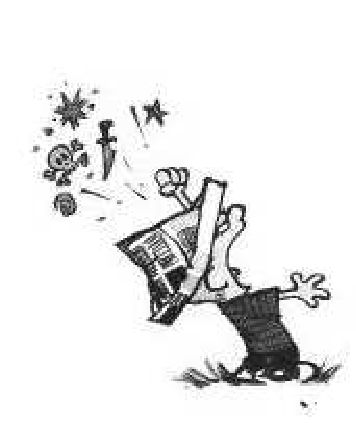
\includegraphics{Images/Chapter/trouble}
\caption{Trouble \ldots}
\label{fig:trouble}
\end{figure}

\blindtext\blindtext

\blindtext


\chapter{Zweites Kapitel}
Um das vorherige Kapitel zu lesen, siehe Kapitel \ref{sec:first}.


\section{Zweite Gliederugsebene...}

Es darf nun weiterer gewichtiger Inhalt folgen.
Hier werden nun einige grundlegenden \LaTeX-Kommandos demonstriert.

\subsection{Dritte Gliederungsebene}

Man kann aber noch tiefer Gliedern

\subsubsection{Vierte Gliederungsebene}

Drei Gliederungsebenen sollten für kleine Artikel und Ausarbeitungen genügen. 
Anderenfalls sollte die Strukturierung nocheinmal überdacht werden.

\paragraph{Paragraph ist die unterste Ebene} \blindtext

\section{Tabellen einbinden}

\begin{table}
\centering
\begin{tabular}{|c||lr|}\hline
1.1 & 1.2 & 1.3 \\ \hline
2.1 & 2.2 & 2.3 \\ \hline \hline
3.1 & 3.2 & 3.3 \\ \hline
\end{tabular}
\caption{Eine simple Tabelle}\label{tab:simple}
\end{table}


Tabellen sollten in einer Table-Umgebung eingefügt und mit einer Caption und einem Label versehen werden.
Ein einfaches Beispiel zeigt Tabelle \ref{tab:simple}.

Leider sind Tabellen eines der schwierigeren Kapitel in \LaTeX,
wenn beispielsweise Zellen zusammengefasst werden.
Tabelle \ref{tab::komplex} zeigt eine etwas aufwendigere Tabelle.


\begin{table}
\centering
\begin{tabular}{c|c|c|c|c|}	
	\multicolumn{2}{c}{}
	& \multicolumn{3}{c}{\begin{scriptsize}\textbf{GdO-Typ}\end{scriptsize}}
	\\ \hhline{~~---}
	\multicolumn{2}{c|}{}
	& \textbf{reellwertig}
	& \textbf{ganzzahlig}
	& \textbf{symbolisch}
	\\ \hhline{~|----}
	\multirow{4}[3]{*}{\rotatebox{90}{\begin{scriptsize}\textbf{EA-Typ}\end{scriptsize}}}
	& \textbf{reellwertig}
	& direkt
	& Rundung
	& ---
	\\ \hhline{~|----}
	& \textbf{ganzzahlig}
	& ---
	& direkt
	& Index
	\\ \hhline{~|----}
	& \textbf{Zeichenkette}
	& Interpretation
	& Interpretation
	& direkt
	\\ \hhline{~|----}
\end{tabular}
\caption{Beispiel für eine komplexere Tabelle}\label{tab::komplex}
\end{table}

\section{Bilder/Grafiken einbinden}

Am besten werden Vektorgrafiken verwendet.
Diese liegen im Idealfall als PDF vor.
Aber auch EPS kann z.B. sehr einfach konvertiert werden.

PDF-Grafiken können unter anderem mit Inkscape \cite{inkscape}, OpenOffice Draw \cite{oodraw} kostenlos bearbeitet und erstellt werden.
Pixelgrafiken sollten unbedingt vermieden werden. 
Ihre Auflösung sollte mind. 300dpi betragen.

\subsection{Einfache Abbildungen}

\begin{figure}
\centering % zentriert alles in der Figure
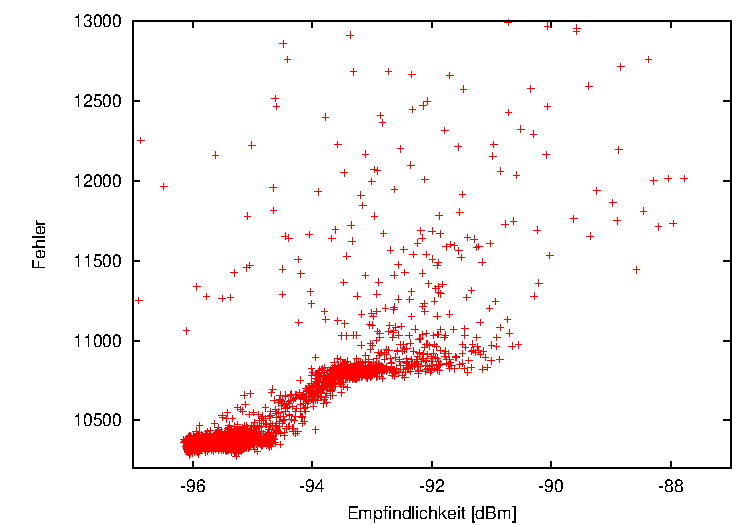
\includegraphics[width=0.6\linewidth]{Images/Chapter/bspgrafik1} % externe Grafik laden
\caption{Dieses Diagramm ist ein Beispiel für eine einfache Abbildung.}\label{fig:testabb}
\end{figure}


Eine Abbildung sollte sich immer in einer Figure-Umgebung befinden.
In dieser kann sie mit einer Caption beschrieben werden
und sie kann über ein Label gekennzeichnet werden (vgl. Abbildung \ref{fig:testabb}).

Dabei muss es keine Grafik sein, die in eine Figure-Umgebung geladen wird.
Es kann dort ganz normal \LaTeX geschrieben werden,
wie Abbildung \ref{fig:testabb2} zeigt.

\begin{figure}
\centering
\fbox{\parbox{0.9\linewidth}{\centering In einer Figure muss keine Grafik stehen... Eine Abbildung kann im Prinzip alles sein.}}
\caption{Dies ist eine Bildunterschrift} \label{fig:testabb2}
\end{figure}

\subsection{Unterabbildungen}

\begin{figure}%
  \centering
   \subfloat[Die erste Unterabbildung]{\label{fig:subfig1}%
       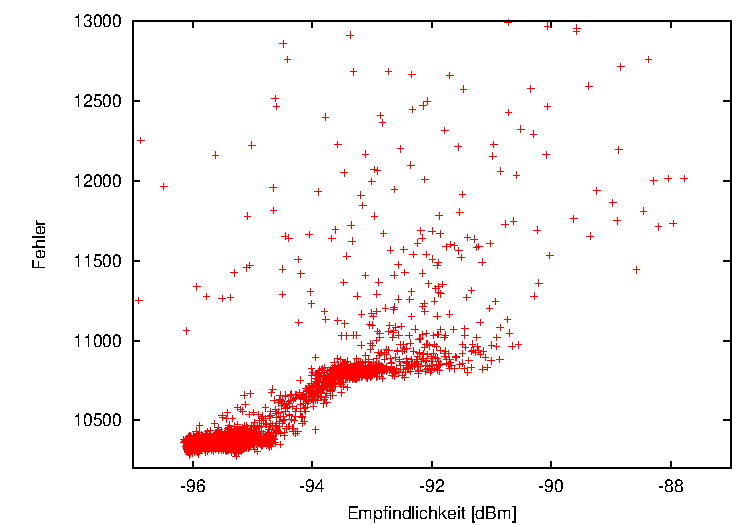
\includegraphics[width=0.48\linewidth]{Images/Chapter/bspgrafik1}
   }\hfill
   \subfloat[Die zweite Unterabbildung]{\label{fig:subfig2}%
       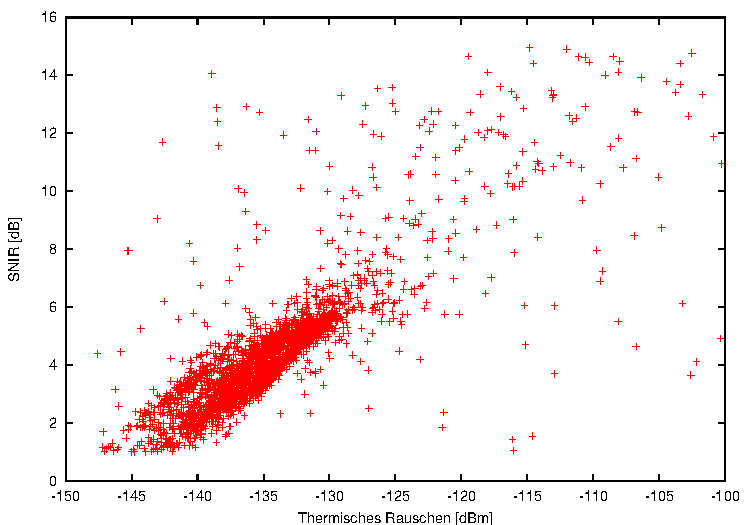
\includegraphics[width=0.48\linewidth]{Images/Chapter/bspgrafik2}
   }
   \caption{Beispiel für Unterabbildungen}
   \label{fig:subfigexample}
\end{figure}


In manchen Fällen ist es sinnvoll eine Abbildung in Unterabbildungen zu teilen.
In Abbildung \ref{fig:subfigexample} wird dies gezeigt.
Die Abbildungen \ref{fig:subfig1} und \ref{fig:subfig2} sind Unterabbildungen.

\section{Formeln}

Für seinen Formelsatz ist \LaTeX besonders bekannt, weshalb es hier nicht an einem kleinen Beispiel (vgl. Formel \ref{eq::gewichtsumme}) fehlen soll.

\begin{equation}
f\idx{sim}(g,U)=\sum\limits^{n\idx{M}}_{\mu=1} w_\mu\cdot c_i( M_\mu(g,U)) \label{eq::gewichtsumme}
\end{equation}

\section{Quelltexte einbinden}

\begin{figure}[t]
\begin{lstlisting}[language=java, caption={Beispiel für ein Listing},  label=lst:bsplst]
public class RadioFitness extends BasicFitness {
  ...
  SimResultReader result = new SimResultReader();
  ...
  protected void readResult(Scenario s) throws FitnessException {
    result.readFrom(s.getExecEnv().getExecutionDir());
  }

  protected double getRawMetric(String name) throws FitnessException {
    if(name.equals("delivery rate")
      return result.getNumSendData()/result.getNumReceivedData();
    else if(name.equals("latency"))
      return results.getLatency();
    else ...
  } // comment
  ...
}
\end{lstlisting}
\end{figure}


Ein Beispiel für ein Java-Listing zeigt Listing \ref{lst:bsplst}.


\section{Zitieren von Quellen}

Aussagen wollen gut belegt sein.
Hier sind willkürlich \cite{FejF08} beispielhafte Zitierungen \cite{Deming1986} angegeben,
die keinen inhaltlichen Bezug zu diesem Text aufweisen.
Vielmehr geht es darum beispielhaft zu zitieren.
Es können auch mehrere Quellen angegeben werden \cite{biturl,Rost2009} (auch hier wieder ohne inhaltlichen Bezug).

Die Literaturangaben werden in einer Datenbank verwaltet,
die in einer .bib-Datei gespeichert wird.
In dieser kann auch nicht zitierte Literatur stehen.
Eine gute Software zur Bearbeitung dieser Datenbank ist JabRef \cite{jabref}.		% Kapitel 1 / n

% ---------------------------Anhang-----------------------------------------
\appendix
\chapter{Source Code Excerpts}


		% Beispielklasse

% ---------------------------Verzeichnisse----------------------------------
\singlespacing 
\bibliography{literatur}	% Literaturverzeichnis
\addcontentsline{toc}{chapter}{\refname}
\listoffigures			% Abbildungsverzeichnis
\listoftables			% Tabellenverzeichnis
\lstlistoflistings		% Codeverzeichnis
\printnomenclature		% Abkürzungsverzeichnis

% ---------------------------Erklärung---------------------------------------
% ---------------------------------------------
% Autor:        Melanie Windrich, Timo Wilgen 
% Vorlage:      Daniel Fötsch, Sven Feja, Eckhard Anders
% Beschreibung: Hauptdatei der Diplomarbeit
% Dateiname:    main.tex 
% Projekt:      Diplomarbeit
% erstellt am:  31.10.2010
% geändert am:  03.04.2017
% SVN:		$Id$
% ---------------------------------------------

\contentspacing

\chapter*{Erklärung}
\label{sec:Erklaerung}
\addcontentsline{toc}{chapter}{Erklärung}

Hiermit erkläre ich,
dass ich die vorliegende Arbeit selbständig und ohne fremde Hilfe angefertigt und keine anderen als die angegebenen Quellen und Hilfsmittel verwendet habe.

% Optionaler Einschub falls der Arbeit die elektronische Fassung beigelegt wird.
\vspace{0.5cm}
\noindent Die eingereichte schriftliche Fassung der Arbeit entspricht der auf dem elektronischen Speichermedium.

\vspace{0.5cm}
\noindent Weiterhin versichere ich, dass diese Arbeit noch nicht als Abschlussarbeit an anderer Stelle vorgelegen hat.




\vspace{30mm}
Kiel, den \today
\vspace{5mm}

\raggedleft \bitAuthor

\end{document}
